 %Premable
\documentclass[11pt]{article}
%List of package
\usepackage{amsmath}
\usepackage{amssymb}  % 수학 툴
\usepackage{graphicx} % Use graphics tool
\usepackage{textcomp} % Use many text symobols
\usepackage{tocloft}  % Add dots for contents
\usepackage{float}    % 그림 그리는데 필요
\usepackage{titlesec} % Chapter 커스터마이징
\usepackage{amsthm}   % Theroem 조판 커스터마이징
\usepackage{fancyhdr} % pagestyle 커스터마이징
\usepackage{ifthen}   % pagestyle 커스터마이징 2
\usepackage{tikz}     % Binomial tree 그리
\usepackage{booktabs} % Table
\usepackage{soul}	  % 밑줄 줄맞춤
\usepackage{breqn}    % 수식 자동 줄맞춤
\usetikzlibrary{arrows.meta} %화살표 그리기
\usepackage{makecell} % node 새로운 줄 
\usepackage[singlelinecheck=false]{caption} %Caption align
\usetikzlibrary{decorations.pathreplacing,angles,quotes} 
\usetikzlibrary{bending}	%Tikzpicture brace 그리기
\usepackage{kotex}
\usepackage{appendix}
\usepackage[normalem]{ulem} % 줄 맞춤 밑줄긋기


% Option of article
\parindent=0cm
\theoremstyle{definition}
\newtheorem{thm}{Theorem}
\theoremstyle{definition}
\newtheorem{lem}{Lemma}
\theoremstyle{definition}
\newtheorem{remark}{Remark}
\theoremstyle{definition}
\newtheorem{lemma}{Lemma}
\theoremstyle{definition}
\newtheorem{prop}{Proposition}
\theoremstyle{definition}
\newtheorem{assume}{Assumption}

\begin{document}
	\begin{center}
		\Large{\textbf{Problem Set \#2}}
		\\~ \\ Heejin Yoon 
		\\~ \\ \small{\today}
		\\~
	\end{center}
	

\section*{Question I.}
\begin{itemize}
\item Individual $i$'s sequential problem can be written as follows: \\
\begin{equation*}
	\begin{split}
		\max_{\{c_{t}^{i}\}}\:&E[\sum_{t=0}^{\infty}\beta^{t}u(c_{t}^{i})]\\
		\text{s.t.}\; &\sum_{t=0}^{\infty}q_{t}c_{t}^{i}=\sum_{t=0}^{\infty}q_{t}(\pi_{e}+0.5\pi_{u}).\\
		\;\\
	\end{split}
\end{equation*}

By taking FOC,
\begin{equation*}
	\begin{split}
	[c_{t}^{i}]:\: & \beta^{t}u'(c_{t}^{i})=\lambda q_{t} \\
	\Rightarrow\: & u'(c_{t}^{i})=u'(c_{t}^{j}) \\
	\Rightarrow\: & c_{t}^{i}=c_{t}^{j}=\pi_{e}+0.5\pi_{u}=\bar{c} \;\; \forall t.\\ 
	\;\\
	\end{split}
\end{equation*}
Also, it is followed by:
\begin{equation*}
	\begin{split}
		& \lambda = \beta^{t}u'(\bar{c})/q_{t}=\beta^{t+1}u'(\bar{c})/q_{t+1}  \\
		\Rightarrow\: & q_{t+1} =\beta q_{t}  \\
		\;\\
	\end{split}
\end{equation*}
Thus, normalizing $q_0=1$, we can obtain $q_t=\beta^{t}$.
	
\end{itemize}


\pagebreak


\section*{Question II.}

\begin{itemize}
\item[a.] The policy function $g(a,s)$ is illustrated below.
\begin{center}
	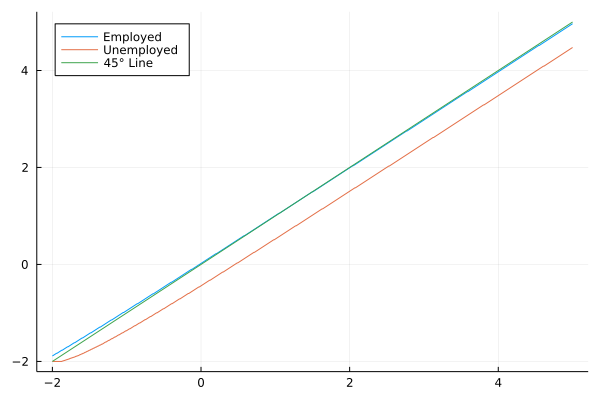
\includegraphics[width=.8\linewidth]{./julia/policy_function.png}
\end{center}
We can obtain $\hat{a}=1.055$ for those employed and $\hat{a}=-2$ for those unemployed.\\
\item[b.] Equilibrium bond price $q$ is equal to $0.99424$. The wealth distributions of the employed and unemployed are drawn below.
\begin{center}
	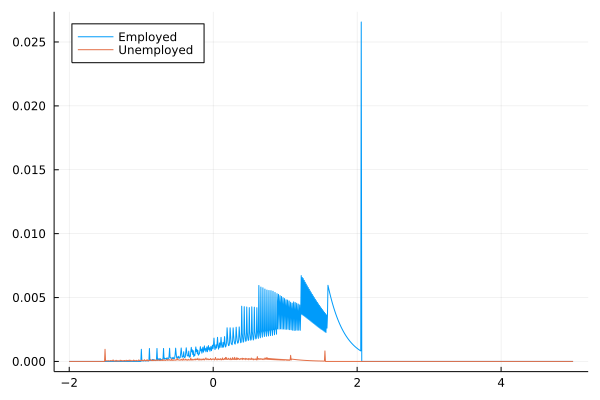
\includegraphics[width=.8\linewidth]{./julia/wealth_distribution.png}
\end{center}
\pagebreak
\item[c.] Lorenz curve is plotted below.
\begin{center}
	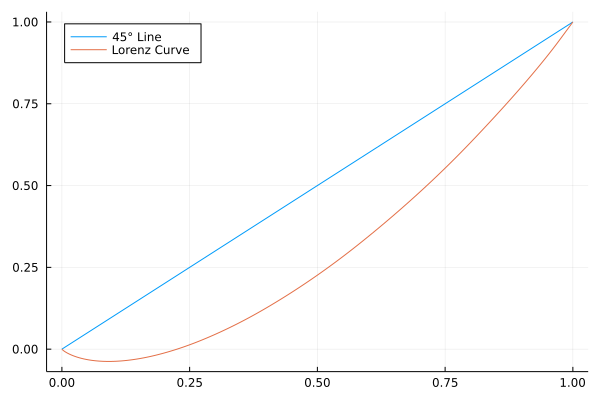
\includegraphics[width=.8\linewidth]{./julia/lorenz_curve.png}
\end{center}
The gini index is 0.38 for this economy. This estimate accounts for about half of the gini index calculated by real world data (0.8).
\end{itemize}	


\pagebreak


\section*{Question III.}

\begin{itemize}
\item[a.] The graphs of $\lambda(a,s)$ for both employed and unemployed people are presented as follows.
\begin{center}
	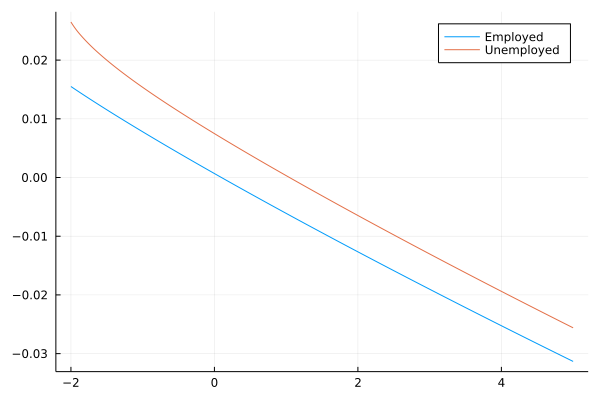
\includegraphics[width=.8\linewidth]{./julia/lambda.png}
\end{center}
\item[b.] $W^{FB}=-4.253$ and $W^{INC}=-4.426$. Thus $WG=W^{FB}-W^{INC}=0.173$.\\

\item[c.] The fraction of the population who favor transforming into complete markets are:
\begin{equation*}
	\sum_{(a,s)\in A \times S} \textbf{1}_{\{\lambda(a,s)\ge0\}}(a,s)\mu(a,s)=0.527
\end{equation*}
\end{itemize}
	
\end{document}